


% Section: Costs and Value Analysis 
\subsection{Cost and Value Relationships in Community Cloud}
\label{sec:costs-value}

The community clouds can be seen as private enterprises with private provisioning of public goods.
This model can suffer from social dilemmas, like the tragedy of the commons, meaning that free riding and under-provisioning will destroy the system in the absence of any mechanisms to overcome these issues.
The socio-economic context of community networks implies that mechanisms that foresee social exclusion can be effective to direct the users' behaviour~\cite{Greiff2013}.


%% Figure 
\begin{figure}[tbp]
	\centering
	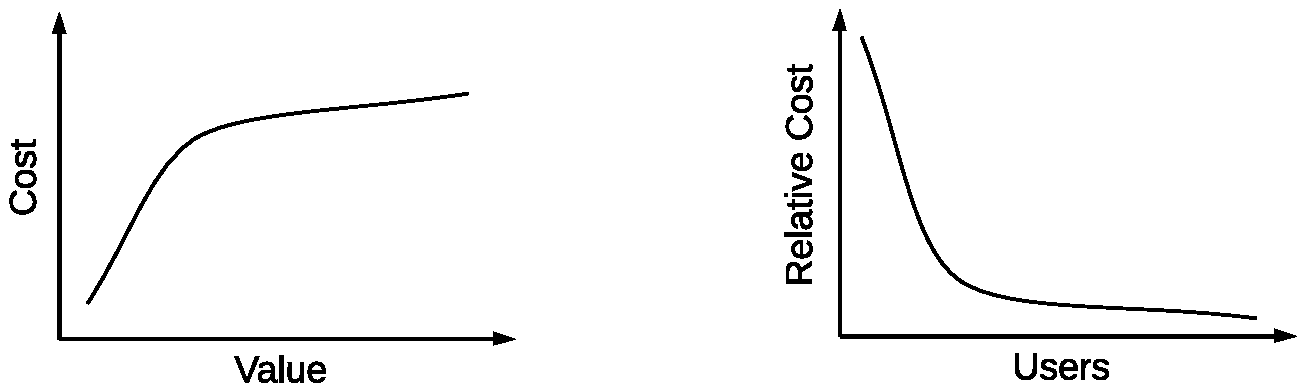
\includegraphics[width=0.75\textwidth, keepaspectratio]{cost-value-relation}
	\caption{Relationship between cost and value in evolution of community cloud}
	\label{fig:cost-value-relation}
\end{figure}

Figure~\ref{fig:cost-value-relation} shows the desired relationship between the cost and value proposition as the community cloud evolves and gets adopted by wider audience.
In the nascent stage, the community cloud will not be able to provide much value until a critical mass of users are using the system.
After that threshold, still the relative cost to achieve a little utility will be significant, which means that the early adopters of the system remain highly motivated and committed to the success of community cloud and continue to contribute resources even though they receive little value from the system in return.
But once a significant proportion of the overall population has joined the community cloud, the relative cost to obtain value from the system tumbles and in the longer run the system is able to sustain itself with contributions that may be small in size but are made by a large number of users.
The objective of the economic mechanisms and the social and psychological incentives is to let the system transition from inception through early adoption to finally ubiquitous usage.


\subsubsection{Costs for Participation}
The initial costs for setting up nodes in the community cloud involves hardware costs including the price of the computing and networking equipment, and installation costs including the manual labour needed.
The continuous operation of the cloud node requires additional costs including network costs given by donating network bandwidth and any other subscription fees, energy costs to pay for electricity bills to run the computer equipment as well as cooling apparatus, maintenance cost to fund any technical support and replacements for parts, and hosting costs to provide storage space for the equipment.
Besides these costs at the individual level, there are also the transaction costs~\cite{Coase1937} or management overheads to direct the group coordination and collaborative production efforts necessary for the operation of community cloud.

\subsubsection{Value Proposition} 
The individuals in community cloud act as private enterprises where they offer services to generate revenue. 
The revenue for the community cloud users include tangible benefits like the services and applications that they will be able to consume, and intangible benefits like the sense of belonging to the community and personal satisfaction because of their contributions.
The services can range from infrastructure to platform to software services meeting a spectrum of different needs of the users.
Once community cloud gets adopted by a critical mass, community may also generate revenue by offering computing resources to commercial enterprises, similar to selling excess power capacity in the case of Smart Grid.
For example, community can get into partnership agreements with the ICT providers where community can buy network bandwidth in return for providing access to the computing resources of the community cloud. 

%
%\subsubsection{Comparison with Commercial Services}
%We discuss the community cloud cost and value in comparison with two popular commercial services that are also based in part on the idea of reciprocal sharing, Spotify\footnote{\url{http://www.spotify.com}} and Skype\footnote{\url{http://www.skype.com}}.
%Spotify is a subscription-based music streaming service which reduces its infrastructure and bandwidth costs by serving cached content from users' devices as well as its own servers.
%Skype is a communication service which uses caches on users' devices for storing and processing information required for managing the underlying infrastructure.
%Both Spotify and Skype offer free as well as paid services. 
%Why do users agree to contribute resources, and even when they are paying for the service?
%
%An argument is that the costs for users are minimal. 
%Both services mostly consume storage, computation time, power and bandwidth on the users' devices. 
%Since these resources are not very expensive and the services' usage remains relatively low, the users do not mind this arrangement or not even notice it.
%But even more important, these services are designed so intuitively that most users do not even realise about donating the resources, and even when they do, the value these services provide has sufficient incentive.
%
%The success of such services implies that for community cloud as well, the users should be able to join with zero or very little costs.
The value proposition of the community cloud services should be strong enough to attract early adopters and keep them committed.
The economic mechanisms in place for encouraging reciprocal sharing and ensuring overall system health and stability should be either invisible for non-technical users or very simple to understand and work with.

